% THIS IS AN EXAMPLE DOCUMENT FOR VLDB 2012
% based on ACM SIGPROC-SP.TEX VERSION 2.7
% Modified by  Gerald Weber <gerald@cs.auckland.ac.nz>
% Removed the requirement to include *bbl file in here. (AhmetSacan, Sep2012)
% Fixed the equation on page 3 to prevent line overflow. (AhmetSacan, Sep2012)

\documentclass{vldb}
\usepackage{graphicx}
\graphicspath{ {images/} }
\usepackage{balance}  % for  \balance command ON LAST PAGE  (only there!)
\usepackage{amsmath}
\usepackage{url}
\usepackage{subcaption}
\usepackage{amsmath}
\usepackage[linesnumbered,ruled]{algorithm2e}
\SetKwRepeat{Do}{do}{while}%


\begin{document}
\newcommand{\argmin}{\operatornamewithlimits{argmin}}
\newcommand{\argmax}{\operatornamewithlimits{argmax}}

% ****************** TITLE ****************************************

\title{ Performance Evaluation of Stream Data Processing Systems}

% possible, but not really needed or used for PVLDB:
%\subtitle{[Extended Abstract]
%\titlenote{A full version of this paper is available as\textit{Author's Guide to Preparing ACM SIG Proceedings Using \LaTeX$2_\epsilon$\ and BibTeX} at \texttt{www.acm.org/eaddress.htm}}}

% ****************** AUTHORS **************************************

% You need the command \numberofauthors to handle the 'placement
% and alignment' of the authors beneath the title.
%
% For aesthetic reasons, we recommend 'three authors at a time'
% i.e. three 'name/affiliation blocks' be placed beneath the title.
%
% NOTE: You are NOT restricted in how many 'rows' of
% "name/affiliations" may appear. We just ask that you restrict
% the number of 'columns' to three.
%
% Because of the available 'opening page real-estate'
% we ask you to refrain from putting more than six authors
% (two rows with three columns) beneath the article title.
% More than six makes the first-page appear very cluttered indeed.
%
% Use the \alignauthor commands to handle the names
% and affiliations for an 'aesthetic maximum' of six authors.
% Add names, affiliations, addresses for
% the seventh etc. author(s) as the argument for the
% \additionalauthors command.
% These 'additional authors' will be output/set for you
% without further effort on your part as the last section in
% the body of your article BEFORE References or any Appendices.

\numberofauthors{8} %  in this sample file, there are a *total*
% of EIGHT authors. SIX appear on the 'first-page' (for formatting
% reasons) and the remaining two appear in the \additionalauthors section.

%\author{
% You can go ahead and credit any number of authors here,
% e.g. one 'row of three' or two rows (consisting of one row of three
% and a second row of one, two or three).
%
% The command \alignauthor (no curly braces needed) should
% precede each author name, affiliation/snail-mail address and
% e-mail address. Additionally, tag each line of
% affiliation/address with \affaddr, and tag the
% e-mail address with \email.
%
% 1st. author
%\alignauthor
%Ben Trovato\titlenote{Dr.~Trovato insisted his name be first.}\\
%   \affaddr{Institute for Clarity in Documentation}\\
%   \affaddr{1932 Wallamaloo Lane}\\
%   \affaddr{Wallamaloo, New Zealand}\\
%   \email{trovato@corporation.com}
%% 2nd. author
%\alignauthor
%G.K.M. Tobin\titlenote{The secretary disavows
%any knowledge of this author's actions.}\\
%   \affaddr{Institute for Clarity in Documentation}\\
%   \affaddr{P.O. Box 1212}\\
%   \affaddr{Dublin, Ohio 43017-6221}\\
%   \email{webmaster@marysville-ohio.com}
%% 3rd. author
%\alignauthor Lars Th{\Large{\sf{\o}}}rv{$\ddot{\mbox{a}}$}ld\titlenote{This author is the
%one who did all the really hard work.}\\
%   \affaddr{The Th{\large{\sf{\o}}}rv{$\ddot{\mbox{a}}$}ld Group}\\
%   \affaddr{1 Th{\large{\sf{\o}}}rv{$\ddot{\mbox{a}}$}ld Circle}\\
%   \affaddr{Hekla, Iceland}\\
%   \email{larst@affiliation.org}
%\and  % use '\and' if you need 'another row' of author names
%% 4th. author
%\alignauthor Lawrence P. Leipuner\\
%   \affaddr{Brookhaven Laboratories}\\
%   \affaddr{Brookhaven National Lab}\\
%   \affaddr{P.O. Box 5000}\\
%   \email{lleipuner@researchlabs.org}
%% 5th. author
%\alignauthor Sean Fogarty\\
%   \affaddr{NASA Ames Research Center}\\
%   \affaddr{Moffett Field}\\
%   \affaddr{California 94035}\\
%   \email{fogartys@amesres.org}
%% 6th. author
%\alignauthor Charles Palmer\\
%   \affaddr{Palmer Research Laboratories}\\
%   \affaddr{8600 Datapoint Drive}\\
%   \affaddr{San Antonio, Texas 78229}\\
%   \email{cpalmer@prl.com}
%}
% There's nothing stopping you putting the seventh, eighth, etc.
% author on the opening page (as the 'third row') but we ask,
% for aesthetic reasons that you place these 'additional authors'
% in the \additional authors block, viz.
\additionalauthors{Additional authors: John Smith (The Th{\o}rv\"{a}ld Group, {\texttt{jsmith@affiliation.org}}), Julius P.~Kumquat
(The \raggedright{Kumquat} Consortium, {\small \texttt{jpkumquat@consortium.net}}), and Ahmet Sacan (Drexel University, {\small \texttt{ahmetdevel@gmail.com}})}
\date{30 July 1999}
% Just remember to make sure that the TOTAL number of authors
% is the number that will appear on the first page PLUS the
% number that will appear in the \additionalauthors section.


\maketitle

\begin{abstract}
Over the past years, Stream data processing is gaining compelling attention both in industry and in academia due to its wide range of applications in various use-cases. To fulfil the need for efficient and high performing  Big data analytics, numerous open source stream data processing systems were developed. Processing data with high throughput while retaining low latency is key performance indicator for such systems. In this paper, we propose a benchmarking system to evaluate the performance of stream  data processing systems, Storm, Spark and Flink  in terms of indicators shown above. More specifically, the latency of windowed aggregation and windowed join operators is evaluated jointly  with the throughput of a system. 
\end{abstract}




\section{Introduction}
Streaming Data Processing (SDP) has been gaining significant attention due to its wide range of uses in Big data analytics. The main reason is that processing big volumes of data periodically is not enough anymore and data has to be processed fast to enable fast adaptation and reaction to changed conditions. Several engines are widely adopted and supported by open source community, such as Apache Storm \cite{toshniwal2014storm}, Apache Spark  \cite{zaharia2012discretized} , Apache Flink \cite{carbone2015apache}. There are definitely, different ways to process stream data before it is persisted in database. For example, while Storm and Flink provide record-by-record stream processing, Spark has a different approach to collect events together and process all in a series of  mini-batches. 


Determining the right  Stream Data Processing System (SDPS) for use case is key to get best performance. Latency and throughput are two main KPIs to measure the performance of SDPS. Latency is the time required to calculate the final result. Because the stream is theoretically infinite and therefore there is no final result, defining latency in SDPS can be tedious. Throughput on the other hand determines the number of successful calculations per unit time. In stream data processing, it is number of tuples source operator can ingest for further process per unit time. 

In this work we propose the benchmark system to assess the performance of three major, open source and community driven streaming engines, being Apache Storm, Apache Spark and Apache Flink.  Throughout  the tests, we use latency and throughput as the major performance indicators. The benchmarks are designed on top of real world use cases, specifically the ones from \textit{Rovio Entertainment}. The  first use case is finding an average price  over numerous streaming data sources by dividing them  into sliding windows. Here, we aim to evaluate the performance of partitioned windowed aggregations. The second use case is comparison of prices which originated in same geo locations by dividing them in sliding windows. Here, we focus on performance of partitioned windowed joins. 

There are numerous works that do benchmarks among different SDPSs with specific Key Performance Indicators (KPI) \cite{perera2016reproducible,chintapalli2016benchmarking}. 
However, researchers in previous works, either don't clearly specify the semantics of KPIs or the determined KPIs are affecting system's actual performance. That is, the definition and calculation of KPIs should be clear and those should be kept separate from system under test.  Moreover, keeping benchmark design simple and with possible less systems, makes the results less biased and reproducible. For example, if one of underlying benchmarking systems is a bottleneck for measurements, then the actual results of system  under test, can be interpreted wrongly. 

TODO: STATEFUL AND STATELESS OPERATORS LATENCY

In this paper, we overcome all of  possible bottlenecks listed above. Our system is generic, has simple design with clear semantics and can be applied to any streaming system. It consists of predefined number of data generators and actual System Under Test (SUT). The link between SDPS and data generator is a socket. To overcome with extra latency of persistent queues, we removed persistent queue as a connector and used sockets. The main intuition is to simulate an environment to get actual latency of a tuple with minimum  affections of other factors. Each tuple has its timestamp field which indicates the time it was generated by data generator. Rather than connecting the SDPS to directly data generator, we put a queue between them as the SDPS may not ingest all generated data. Waiting in queue increases the latency of a tuple, so the sooner the system pulls data from queue, the lower the latency will be. The throughput on the other hand, is calculated by number of pulls of SDPS to queue in a unit time. 

The main contributions of this paper are listed above:
\begin{itemize}  
\item In this paper, we  introduce  the first mechanism to measure the latency in stateful operators is SDPS. We applied the proposed method with partitioned windowed aggregation and partitioned windowed join use cases. 
\item The proposed benchmarking system measures the throughput of a system and the latency of an operator out of the box. That is, the throughput is associated with the system and therefore we measure throughput outside the system, in data generator module. Moreover, the latency is linked with operator, therefore, we assess it outside of operator. The main goal is, to eliminate side factors affecting the measurements. 
\item Because we are testing SDPSs, the backpressure is an inportant feature for such systems and should be considered. We introduce the first solution to check the SUT's upper limit of throughput taking into consideration backpressure and system initialization delays. If the system cannot sustain the data rate, depending on user's configuration,  data-queue module will tolerate it for some time.
\item We test the SDPSs with different  configurations and cluster size and provide the analysis of the experimental results.
\end{itemize}

The remainder of paper is organised as follows. In Section ... TODO

\section{Related work}
The main concepts and methodologies used in benchmarking SDPS were inherited from big data benchmarks.
Now with emerging next generation stream data processing engines, batch processing is seen as a special case of stream processing where the data size is bounded. Huang et.al. propose HiBench, the first benchmark suite for evaluation and characterisation of Hadoop \cite{white2012hadoop}. Authors conduct wide range of experiments from micro-benchmarks to machine learning algorithms \cite{huang2011hibench}. Covering end-to-end big data benchmark with all major characteristics such as three Vs in the lifecycle of big data systems is the main intuition behind BigBench \cite{ghazal2013bigbench}. Wang et.al. introduce BigDataBench, a big data benchmark suite for Internet Services, characterising the 19 big data benchmarks covering broad application scenarios and diverse and representative data sets \cite{wang2014bigdatabench}.

 Benchmarks on SDPS are  Researchers from Yahoo Inc. have done benchmarks on streaming systems to measure latency and throughput \cite{chintapalli2016benchmarking}. They used Apache Kafka \cite{kafka2014high} and Redis \cite{carlson2013redis} for data fetching and storage. Later on, on the other hand, Data Artisans, showed those systems actually being a bottleneck for SUT's performance \cite{dataartisans}.  The extensive analysis of the differences between Apache Spark and Apache Flink in terms of batch processing is done by correlating the operators execution plan with the resource utilization and the parameter configuration \cite{marcu2016spark}. In another benchmark, authors compare the performances of Apache Spark and Apache Flink to  provide clear, easy and reproducible configurations that can be validated by community in clouds \cite{perera2016reproducible}. Authors conducted  benchmarks to assess the fault tolerance and throughput efficiency for open source stream data processing engines \cite{lopez2016performance}. In another benchmark, authors motivate IoT as being main application area for SDPS and perform common tasks in particular are with different stream data processing engines and evaluate performance \cite{shukla2016benchmarking}. One of the pioneers in SDPS benchmarks, developed framework StreamBench analysing the current standards in streaming benchmarks and proposing a solution to measure throughput, latency considering the fault tolerance of SUT \cite{lu2014stream}. Authors put a mediator system between data generator module and SUT and define the latency as the average time span from the arrival of a record till the end of processing of the record. LinearRoad benchmarking framework was presented by Arasu et al. to measure performance of standalone stream data management systems such as Aurora \cite{abadi2003aurora} by simulating a scenario of toll system for motor vehicle expressways. Several stream processing systems implement their own benchmarks to assess the performance \cite{neumeyer2010s4,qian2013timestream,zaharia2012discretized}. SparkBench is a benchmarking framework to evaluate machine learning, graph computation, SQL query and streaming application on top of Apache Spark \cite{li2015sparkbench}.


\section{PRELIMINARY AND BACKGROUND}


In this section we provide preliminary and background information about the stream data processing engines used throughout this paper.  Initially, the general information about the working principles of particular system is given.  Afterwards, we provide more use case specific info for each system. Because we test engines' partitioned windowed join and  aggregation operators, basic semantics of particular operators , computational model and back-pressure mechanism are analysed.  
\subsection{Apache Storm}

Apache Storm is a distributed stream processing computation framework which was open sourced after being acquired by Twitter. 


\textbf{Computational model}
Storm operates on tuple streams and provides record-by-record stream processing. It supports at-least-once processing (when there are failures events are replayed) mechanism and guarantees all tuples to be processed. Storm also supports exactly-once semantics with its Trident abstraction. The core of Storm data processing is a computational topology which consists of spouts and bolts.  Spouts are source operators whereas bolts are processing and sink operators. Because Storm topology is DAG structured, where the edges are stream tuples and vertices are operators (bolts and spouts), when a spout or bold emits a tuple, the ones that are subscribed to particular spout or bolt receive input. Storm's parallelism model is based on \textit{tasks}. Each task runs in parallel and by default single thread is allocated per task. 

Storm's lower level API's provide little support for managing the memory and state. Therefore, choosing the right data structure for state management, utilizing memory usage efficiently my making computations incrementally  is up to the user. 
memory management. Storm supports cashing and batching the state transition. However, the efficiency of particular operation degrades as the size of state grows.  Storm  supports back-pressure.



\textbf{Windowing}.
Storm has built-in support for windowed calculations. That is, partitioned windowed joins and aggregations are supported internally.  Although the information of expired, new arrived and total tuples within window is provided through APIs, the state management and making computations incremental  should be done manually. Storm supports processing and event-time windows with sliding and tumbling window features. Processing time windows include time and count based semantics. For event-time windows, tuples should have separate timestamp field so that the engine can create periodic watermarks. One of the downsides of Storm's relying heavily on ackers, is that tuples can be acked once they completely flush out of window. This can be an issue specially, on windows with big length and small slide.  



\subsection{Apache Spark}
Apache Spark is an open source data processing engine, originally developed at the University of California, Berkeley. 

\textbf{Computational model}
Spark internally is batch processing engine. It handles the stream processing by micro-batches. As can be seen from Figure \ref{fig_micro_batch},  Spark Streaming resides at the intersection of batch and stream processing.  Resilient Distributed Dataset (RDD) is a fault tolerant abstraction which enables in memory parallel computation in  distributed cluster environment \cite{zaharia2012resilient}. Unlike Storm and Flink, which support one record at a time, Spark Streaming inherits its architecture from batch processing which support processing records in micro-batches. 

One of Spark's features is that it supports lazy evaluation and tries to  limit the amount of work it has to do. This enables the engine to run more efficiently. Spark also supports DAG based execution graph which works implementing  stage-oriented scheduling. Unlike from Flink and Storm, which also work based on DAG exetuion graph, Spark computing unit in graph is data set rather than streaming tuple and each vertex in graph is a stage rather than operators. RDDs are guaranteed to be processed in order in a single DStream. However, the order guarantee within RDD is not provided since each RDD is processed in parallel. 

Spark Streaming has improved significantly its memory management in recent releases.  The memory is shared between execution and storage. This unified memory management supports dynamic memory management between the two modules. Moreover, Spark supports dynamic memory management throughout the tasks and within operators of each task. 

\textbf{Windowing}
Spark Streaming has a built-in support for windowed calculations. Processing time windows with sliding and tumbling versions are  supported in Spark. The operations done with sliding windows, are internally incrementalized transparent to the user.  However, choosing the length batch interval can affect the window based analytics. Firstly, the latency and response time of windowed analytics is strongly replying on batch interval. Secondly, supporting only processing time windowed analytics, can still be a bottleneck in some use cases. Spark supports back pressure which is very useful in windowed calculations. The window size must be a multiple of the batch interval, because window keeps the particular number of batches until it is purged. 




\subsection{Apache Flink}
Apache Flink which was started off as an academic open source project (Stratosphere \cite{alexandrov2014stratosphere}) in Technical University of  Berlin.

\textbf{Computational model}
Distributed dataflow engine is standing in the core of Flink. It is responsible for executing the dataflow programs. Like Storm, A Flink runtime program is a DAG of stateful operators connected with data streams. Flink's runtime engine supports unified processing of batch (bounded) and stream (unbounded) considering former as being the special case of the latter.

Flink provides its own memory management to avoid long running JVM's garbage collector stalls by serialising data into memory segments. 
The data exchange in distributed environment is done via buffers. So, producer takes a buffer from the pool, fill it up with data, and the consumer receives data and frees the buffer informing the memory manager. There are different mechanisms such as sending when buffer is full or sending when timeout is reached to link buffers between consumer and producer or sending locally or remotely. Flink provides wide range of high level and user friendly APIs to manage the state. The incremental state update, managing the memory or checkpointing with big states is done automatically, transparent to user. 

\textbf{Windowing}
Flink owns strong feature set for building and evaluating windows on data streams. With wide range of pre-defined windowing operators, it supports user defined windows with custom logic. The engine provides processing time, event time and ingestion notion of time.  In processing time, like Spark,  windows are defined with respect to the wall clock of the machine that is responsible for building and processing  a window. In event time on the other hand, the notion of time is  determined when the event are created. Like in Storm, the timestamps must be attached to each event record as a separate field. In ingestion time, the system still processes with event time semantics but on the timestamps which were assigned when tuples arrive the system. Flink has a support for out-of-ordered streams which gained popularity after Googles MilWheel and Dataflow papers \cite{akidau2013millwheel,akidau2015dataflow}


\begin{figure}[h]
\centering
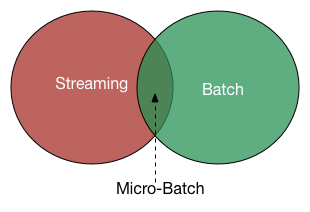
\includegraphics[width=0.35\textwidth]{streambatch}
\caption{Conceptual view of micro-batching}
\label{fig_micro_batch}
\end{figure}


\section{Challenges}
There are several challenges to be taken into consideration while designing a benchmark for SDPSs. In this section we analyse the challenges and provide solutions.

\textbf{ \textit{Simple is beautiful}}. The first challenge is to design a simple system, because simple is beautiful. As the number of systems included inside benchmark increases, the complexity escalades at the same time. One of downsides of the complex system is, difficult to determine the bottleneck. For example, to test the stream data processing engine, the data generator component is essential, to simulate the real life scenarios. Figure \ref{fig_queue_link} shows possible three cases to link data generator and SUT. The simplest design would be connecting the SDPS directly to data generators as shown in Figure \ref{fig_no_queue}. Although this is perfectly acceptable case, it confronts with real life use cases. That is,  in real life, the stream data processing engines, do not connect to pull based data sources unless there is a specific system design. Usually, SDPSs pull data from the distributed message queues which reside between data generators and SUT. One bottleneck on this option is throughput which is bounded by the maximum throughput of message queueing system. We selected the third option which stands between the first two. As can be seen from Figure \ref{fig_partial_queue}, we embedded the queues as a separate module in data generators. In this way, the throughput is bounded only by network bandwidth, the system works more efficient as there are no se/deserialisation overheads and finally it has a simple design. Moreover, while measuring the performance of SUT, using extra systems for checkpointing the current state of measurements or for saving the intermediate evaluation results can affect the SUT's performance.


\textbf{ \textit{Keep driver and test unit as separate as possible}}. The second challenge is to isolate the benchmark driver and SUT as much as possible. For example, in benchmarking SDPSs, it is common to measure the throughput inside the SUT. Because both computations can affect each other the results can be  biased  which we discuss below. We solved this problem by categorising the test unit and pointing measurements accordingly. The first evaluation is throughput. Throughput is associated with the system. So, we kept the throughput assessment outside the SUT, inside data generator module. The second evaluation is latency. The latency is linked with an operator inside system. So, we kept all latency measurements outside the particular operator.

\textbf{ \textit{ Avoid misleading tests}}.
The third challenge is abstain from biased test results and keep the evaluation semantics clear.  One example for this is, throughput measurement. In the previous SDPS benchmarks, the throughput of a SUT is measured by either taking quantiles over test time, or showing max, min and average assessments. From user's perspective on the other hand, the system's throughput is the one with upper bound that it can sustain the data processing. When conducting the experiments with stream data processing engines, back pressure is another factor affecting the throughput, that should be taken into consideration.  Another example for this challenge is latency measurement. In the previous SDPS benchmarks, the latency of an operator is measured by taking difference of tuple's ingestion timestamp to system and output timestamp from system. However, from user's perspective, the start timestamp of a tuple is once it is created and latency of particular tuple should be calculated by taking into consideration its event timestamp. We solve the first issue by measuring the SUT's max throughput that it can sustain under back pressure with a given amount of input. We developed the mechanism for handing the back pressure.  For the second issue, we measure the latency of a tuple by differentiating the time when output is done and its event timestamp.


\textbf{ \textit{ Latency of stateful operator?}} The fourth challenge is measuring the latency of stateful operator. Up to this point, the related works in literature either concentrated on stateless operators or evaluated the latency of stateful operators by checkpointing to external systems like lightweight distributed databases. As we discussed above, this approach can be a bottleneck in some cases. In this paper, we provide a solution for this problem without any external system. 


\begin{figure*}
    \centering
    \begin{subfigure}[b]{0.32\textwidth}
        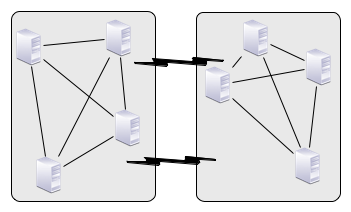
\includegraphics[width=\textwidth]{no_queue}
        \caption{Without message queue}
        \label{fig_no_queue}
    \end{subfigure}
    ~ %add desired spacing between images, e. g. ~, \quad, \qquad, \hfill etc. 
      %(or a blank line to force the subfigure onto a new line)
    \begin{subfigure}[b]{0.32\textwidth}
        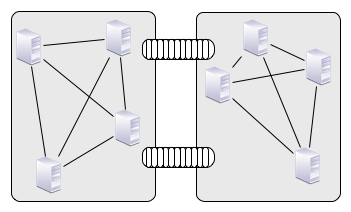
\includegraphics[width=\textwidth]{yes_queue}
        \caption{With message queue}
        \label{fig_yes_queue}
    \end{subfigure}
    ~ %add desired spacing between images, e. g. ~, \quad, \qquad, \hfill etc. 
    %(or a blank line to force the subfigure onto a new line)
    \begin{subfigure}[b]{0.32\textwidth}
        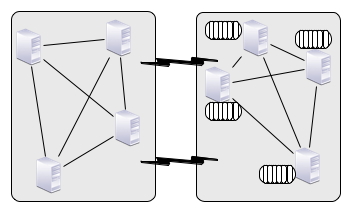
\includegraphics[width=\textwidth]{node_queue}
        \caption{Partial message queue}
        \label{fig_partial_queue}
    \end{subfigure}
    \label{fig_queue_link}
        \caption{Different system designs to link data generator and SUT.}
\end{figure*}



\section{Benchmark system design}
We keep overall design of benchmark simple. Figure \ref{fig_design} shows the overall intuition behind the benchmark system. There are two main components of a system:
\begin{itemize}  
\item SUT
\item Data Engine 
\begin{itemize}  
      \item Data Generator
       \item Data Queue
\end{itemize}

\end{itemize}

The Data Engine component is responsible for generating and queueing the synthetic data. It has two subcomponents: Data Generator and Data Queue. Both of them reside in the same machine to avoid network overhead and the data is kept in memory to circumvent the disk write/read overhead. First subcomponent, data generator, generates data with a given speed. To ensure high throughput we kept the number of fields in an event minimal. To assure the scalability and each Data Generator connects to its own Data Queue rather than to common and centralized message queue. Queue is based on FIFO semantics. In this way, we avoid data de-/serialization, disk read/write and network overhead. Theoretically, this approach has no difference from the one  which includes centralized and distributed message queue. The following analogy can be made: the topic in distributed message queueing system is analogous to Data Queues, and partition is single Data Queue. The Data Generator appends the current time to timestamp field of an event. The event's latency is calculated from this point and the more it stays in queue, the more the latency is. The number of Data Engines can be arbitrary and its overall throughput is only bounded by network bandwidth. As we discussed above, the throughput assessment which is associated with the SUT as a whole,  is done in Data Engine component, which has a clear separation from SUT. 

The SUT is second main component, which processes the data. So the only interface of Data Engine to outer world is Data Queue subcomponent. SUT pulls data from Data Queue. The connection is pull based because we let the SUT to decide when and how much data it can ingest. The SUT connects predefined number of Data Queues. Firstly it combines the input data sources. There can be one or two unions, depending on the operator semantics. For example, windowed aggregation is a single input stream (union of streams) operator but join operator accepts two streams (union of streams) as an input. The latency calculation is done inside SUT. This measurement is associated with the operator inside SDPS, we clearly separate the latency assessment from Operator Under Test (OUT). Placing extra stateless operator just after OUT and measuring the latency between the event time and current time gives the latency of an element. The calculation of latency in windowed aggregation and windowed join operators is shown in Section \ref{sec_latency}. 


%Proper handling tuples' timestamp fields while joining or aggregating is crucial. In this work, \textit{merging} of tuples' timestamp fields is done by selecting \textit{maximum} over them. That is, latest arrived tuple's timestamp is transferred to the new tuple as a result of aggregation or join. Equation \ref{eq_1} defines this logic formally.
%
%
%Here $t \in T$ is a stream tuple,  $t[k]$ is  $k^{th}$ field of particular data point and $\equiv$ means equivalent in terms of type. For aggregation function $|T|$, the size of a set is not bounded, whereas for join function it is bounded by two, being $|T| = 2$.

\begin{figure*}[h]
\centering
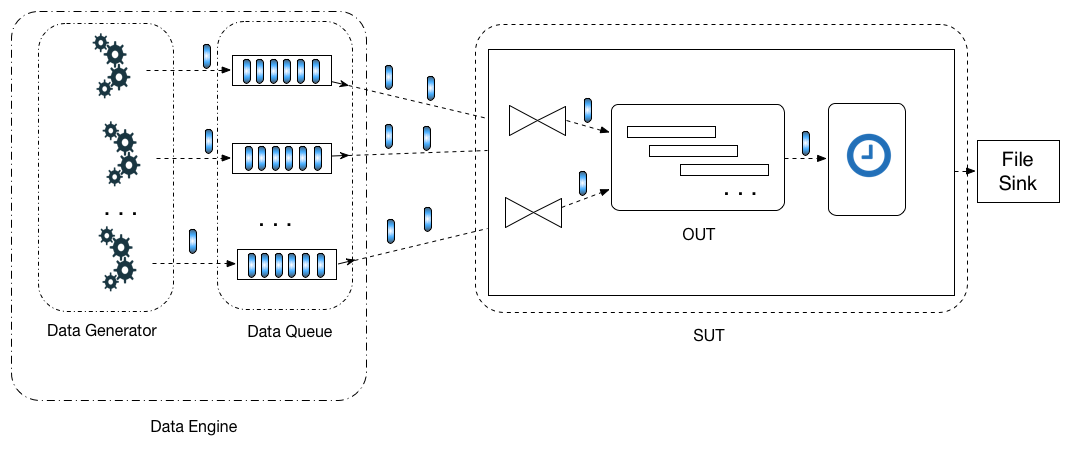
\includegraphics[width=1\textwidth]{system_design}
\caption{Design of benchmark system.}
\label{fig_design}
\end{figure*}

\subsection{Use case}
The use case for this benchmark is provided by \textit{ Rovio Entertainment}. It is known as a video game development company. To get higher customer satisfaction, it is mandatory to analyse the game usage statistics. For example, company releases a new feature for a particular video game. It is essential to have a quick overview of customer's opinion by analysing the usage statistics. For that reason, Rovio uses stream data processing analytics rather than batch based periodic analysis.  In all use cases an event has following fields: event timestamp, key and value. 

\textbf{Windowed Aggregation}
Windowed aggregations are important part of the statistics analytics from the feed stream. One use case is computing the user average session time within windows. Each event has its geo ID, which indicate the location in which an event was generated. A use case includes partitioning the events by their ID and finding the average session time within windows. Here, the key field is geo location and value field is session time. Another use case is computing the average ads screening time within window for each geo location. 

\textbf{Windowed Join}
Joining several stream feeds based on key field within window is another general use case for user statistics analytics. One specific use case is joining two user statistics stream feed within window by geo field and calculating an event with higher session time and the difference between them. In this use case the key field would be geo location and value would be the session time. Another use case would be doing the same procedure with ads watch time. 


\subsection{Key Performance Indicators}
The Key Performance Indicators ( KPIs) for this benchmark are latency and throughput. The throughput indicator is related with SUT, on the other hand, the latency is associated with OUT. 


%To measure the performance of a system, we connected max $16$ data generators to system under test with order of $1$,$2$,$4$,$8$ and $16$ as increasing further does not increase the overall throughput significantly. We call the tests with related workloads as $1x$, $2x$, $4x$, $8x$ and $16x$. Moreover, the configuration of each data generator must be the same. Configuration includes parameters such as overall input size, generation speed, socket port and etc. Equation \ref{eq_2} defines this formally.
%
%\begin{equation}
%  \begin{gathered}
% \textbf{Let} \ d_{i}^{c_{i}} \in  D\\
%  \textbf{then}, |D| \gets S \\
%  \textbf{and} \ c_{1} = c_{2} \ ... = c_{n}, \forall n \in S = {1,2,4,8,16}
%  \end{gathered}\label{eq_2}
%\end{equation}


\subsubsection{Throughput}
\textit{Definition.  Let $c_{i} \in C$ be a configuration for a Data Engine, $d_{i} \in D$,  $c_{i}^{sp}$ be the data generation speed configuration which can be sustained by SUT. If  $\exists c_{i} \in C$ such that $c_{1} = c_{2}... = c_{i}$ and  $T = \sum_{i}c_{i}^{s}$ is maximum, $\forall c_{i} \in C, \forall i \in \{1,2,3 ... |C|\}$, then $T$ is a maximum sustainable throughput of SUT.}

Throughput of a system is calculated as summing the throughout of each Data Engine  because the SUT is expected to pull the data from all Data Queue subcomponent of Data Engine approximately with same rate. We restricted the configuration of all Data Engines to be the same, to ease calculating the maximum sustainable throughput. It is crucial to note that the maximum sustainable throughput is not the same as maximum throughput of Data Engine but the one for SUT. 

To examine the system's sustainability with a given throughput, we divide the queue used in Data Queue subcomponent into three parts: $c^{a}$ , $c^{b}$ and $c^{n}$. The Figure \ref{fig_queue}, shows the example partitioning of queue. If the size of the queue is less than or equal to $c^{a}$ then this is acceptable and means, the SUT can sustain the given throughput. If the queue size is less than or equal to $c^{b}$ on the other hand, the SUT cannot sustain the given data rate but we can tolerate it for some time, in case the increase in queue size is an outcome of back-pressure. However, if the queue size is bigger than the $c^{b}$ then the SUT cannot sustain the given throughput and there is no need to do benchmarks with particular data rate.

The semantics behind  examination of SUT's sustainability with a given throughput must be clear. Moreover, it should support the system specific behaviours like back-pressure. Algorithm \ref{alg_sustainable} show an algorithm to check if the  SUT can sustain  the given throughput of a single Data Engine. It gets the configuration $c$ of Data Engine as an input. After firing the Data Engine with configuration $c$, in line $3$, it is put to $idle$ position, meaning no data is generated until the SUT makes its first data pull request from Data Queue subcomponent. $c^{input}$ is the input count that must be generated in particular Data Engine.
 In lines $10-11$ the events are generated with speed $c^{sp}$ in Data Generator subcomponent of Data Engine component and put into the queue of Data Queue subcomponent. We check the queue size periodically, once per $c^{a}$ element and not for each iteration. The first reason is that the data pull rate of stream data processing engine is not steady and therefore checking the queue size with little delays makes more sense. The second reason is that, $c^{a}$ can be thought of the $confidence limit$ as shown in Figure \ref{fig_queue}. While checking the queue size there are three possibilities. The first is (lines $13-15$), the size is bigger than $c^{b}$, the back-pressure limit. In this case, the Data Engine is stopped and the $false$ is returned meaning the SUT is not sustainable with given throughput. The second is (lines $16-18$), queue size is less than $c^{a}$, the acceptable queue size. In this case, we set back-pressure counter to zero, in case there was one and continue generating data. The third is (lines $19-23$), the size   of queue is within boundaries of $c^{a}$ and $c^{b}$. In this case, we can tolerate the SUT for at most $\frac{c^{b}}{c^{a}}$ times. If the system can pull the data in queue and set the size of queue within \textit{confidence} boundaries ($c^{a}$) in a given period, then it continues, else, the application returns $false$ meaning, the SUT cannot sustain the given throughput. 

\begin{algorithm}
    \SetKwInOut{Input}{Input}
    \SetKwInOut{Output}{Output}

    \underline{function isSustainable} $(c)$\;
    \Input{ $c$ is configuration of Data Engine}
    \Output{return $true$ if is sustainable, $false$ otherwise}
    Fire Data Engines with configuration $c$. \\
    $c^{st} \gets idle$  \tcp*{wait for SUT to pull data}
  \While{There is no pull request from SUT}{
    wait \\ 
   }    
       $c^{st} \gets active$ \tcp*{start generating data}
       $bp\_index \gets 0$ \tcp*{initialize back-pressure index}
       \For{$i \gets 0; i < c^{input}; i++$}{
       Generate $e_{i} \in E$ with speed $c^{sp}$\\
       queue.put($e_{i}$) \tcp*{put  generated event to queue}
        \tcc{check the queue once per $c^{a}$ elements}
        \uIf{i \% $c^{a} == 0$}   { 
               \uIf{ $queue.size > c^{b}$  }   { 
              		Stop Data Engine \\
		         return $false$
               }
               \uElseIf{  $queue.size < c^{a}$ }{
               $bp\_index \gets 0$ \tcp*{ no back-pressure} 
               $continue$ \tcp*{SUT can sustain so far} 
               }
               \uElse{ 
                \tcc{ Tolerate for back-pressure}
                  $bp\_index \gets bp\_index +1$ \\
                     \uIf{$bp\_index == \frac{c^{b}}{c^{a}}$}{
                       \tcc{ This is not back-pressure}
                        Stop Data Engine \\
		         return $false$  
                     }
               }
        }
       }
    \caption{Throughput sustainability test of single data engine}
    \label{alg_sustainable}
\end{algorithm}

\textit{Definition.  Let $c_{i} \in C$ be a configuration for a Data Engine, $c_{i}^{dr}$ be a data generation rate of particular Data Generator, $d_{i} \in D$ and $n$ be the number of Data Engines being $n = |D|$.  The SUT is sustainable with given throughput $n * c_{dr}$,  $iff$ $isSustainable(c_{i})  == true$ $\forall$ $i \in \{1,2,3,...n\}$}

The above definition states that the SUT is sustainable with a given data generation rate iff, it can sustain all Data Engines at the same time. If one of the Data Engines cannot be sustained, then SUT is said is not sustainable with a given data generation rate. 


\subsubsection{Latency}
\label{sec_latency}
Latency is another KPI for this benchmark and defining the latency needs clear semantics. There are several points that needs to be clarified: \textit{i)} the aggregation or join of timestamp fields of tuples and \textit{ii)} clear boundaries (start and end timestamp) of latency.

The first point is the aggregation or join of tuples with timestamp fields. While the use case provides the semantics for aggregating or joining the tuples' $value$ fields, the one for timestamp field is unclear. For example, in windowed aggregation operator, which calculates the average of elements' $value$ field, the aggregation semantics with tuples' timestamp field is unclear.  The Equation \ref{eq_1} addresses this issue. Let $t[k]$ and $t'[k]$ denote the timestamp field for tuples $t$ and $t'$ respectively,  $\equiv$ be an operator checking for the type and $TS$ be tuple field of type timestamp. Here, $f_{s}$ is an stateful operator which takes a set of tuples $t \in T$ and converts it to tuple $t'$. Then there exists $k$ and $m$ such that the respective fields of input and output tuples have the same type being timestamp and the output tuple's timestamp is calculated taking maximum among input tuples. Here input and output tuples are associated with operator $f_{s}$ and not with the SUT.

The calculate the latency, it is crucial to have clear boundaries of when to start and stop the stopwatch for each tuple. Equation \ref{eq_2} defines the basic semantics behind this. This is basically a follow-up for Equation \ref{eq_1}. Let $t_{i} \in I$ be a tuple in input set and $t_{o} \in O$ be a tuple in output set. The latency is associated with output tuples. So, the latency of tuple $t_{o}$ is calculated by extracting the $t_{o}[m]$, the timestamps field from current time. The calculation of output tuples' timestamp field is shown in Equation \ref{eq_1}. 


\begin{equation}
  \begin{gathered}
\textbf{Let} f_{s}:\{t| t\in T \} \to t'  , \\
  \textbf{then}, \exists k,m \ s.t. \ t[k]  \equiv t'[m] \equiv \ TS \ \forall t \in T\\
  \textbf{and} \ t'[m] \gets \argmax\{t[k] \ | \ t \in T\}  
    \end{gathered}
      \label{eq_1} 
  \end{equation}

   \begin{equation}
     \begin{gathered}
  \textbf{Let} \ t_{i} \in I , t_{o} \in O \\
\textbf{then} \ Latency_{ \ t_{o}} = time_{now} -  t_{o}[m] \\
s.t. \ f_{s}:\{t_{i} \ | t_{i} \in I \} \to \{t_{o} \ | t_{o} \in O \} \\
\textbf{and} \ t_{o}[m] \equiv TS
  \end{gathered}
  \label{eq_2} 
\end{equation}



\begin{figure}[h]
\centering
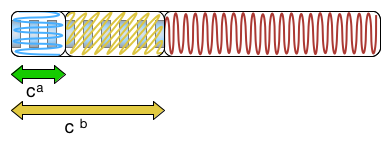
\includegraphics[width=0.45\textwidth]{queue}
\caption{Basic intuition behind \textit{back-pressure-compatible queue}}
\label{fig_queue}
\end{figure}


\section{Evaluation}
\subsection{Configuration}
The following configurations are used throughput experiments:
\begin{itemize}
\item Cluster size: 2,3,4 and 8 node clusters
\item Parallelism within single node: number of cores, which is 16.
\item Parallelism within cluster: (Parallelism within single node) * (number of nodes)

\item Backpressure: enabled in all systems
\item Network bandwidth: 1Gb
\item Number of Data Engines running in parallel: 16
\item Allocated memory: 16GB
\item Cluster type: Standalone
\item Input size for aggregation use case: 150M * 16
\item Input size for join use case: 
\item Spark batch size: 4 seconds and 2 seconds
\item Window type: Processing time
\item Number of distinct keys in input: 160
\item Join inputs selectivity: 
\item $c_{a}$, acceptable queue limit: 1M
\item $c_{b}$ backpressure tolerated queue limit: 15M
\end{itemize}

\subsection{Keyed Windowed Aggregations}
scale up/down

window size increase/decrease

batch siez increase/decrease

\subsection{Joins}
same as above
\section{Conclusions}
%\end{document}  % This is where a 'short' article might terminate

% ensure same length columns on last page (might need two sub-sequent latex runs)
\balance

%ACKNOWLEDGMENTS are optional
\section{Acknowledgments}


% The following two commands are all you need in the
% initial runs of your .tex file to
% produce the bibliography for the citations in your paper.
\bibliographystyle{abbrv}
\bibliography{vldb_sample}  % vldb_sample.bib is the name of the Bibliography in this case
% You must have a proper ".bib" file
%  and remember to run:
% latex bibtex latex latex
% to resolve all references


%APPENDIX is optional.
% ****************** APPENDIX **************************************
% Example of an appendix; typically would start on a new page
%pagebreak






\end{document}
